\documentclass[openany]{book}
% useful packages, copy and paste from diff sources
\usepackage[english]{babel}
\usepackage[T1]{fontenc}
\usepackage{cite,url,color} % Citation numbers being automatically sorted and properly "compressed/ranged".
\usepackage{graphics,amsfonts}
\usepackage{epstopdf}
\usepackage[pdftex]{graphicx}
\usepackage[cmex10]{amsmath}
\usepackage{algorithm, algorithmic}
\usepackage{subfigure}
% Also, note that the amsmath package sets \interdisplaylinepenalty to 10000
% thus preventing page breaks from occurring within multiline equations. Use:
\interdisplaylinepenalty=2500
% after loading amsmath to restore such page breaks as IEEEtran.cls normally does.
\usepackage[utf8]{inputenc}
% Useful for displaying quotations
%\usepackage{csquotes}
% Compact lists
%\let\labelindent\relax
\usepackage{enumitem}

%tikz figures
\usepackage{tikz}
\usetikzlibrary{automata,positioning,chains,shapes,arrows}
\usepackage{pgfplots}
\usetikzlibrary{plotmarks}
\newlength\fheight
\newlength\fwidth
\pgfplotsset{compat=newest}
\pgfplotsset{plot coordinates/math parser=false}

\usepackage{array}
% http://www.ctan.org/tex-archive/macros/latex/required/tools/
%\usepackage{mdwmath}
%\usepackage{mdwtab}
%mdwtab.sty	-- A complete ground-up rewrite of LaTeX's `tabular' and  `array' environments.  Has lots of advantages over
%		   the standard version, and over the version in `array.sty'.
% *** SUBFIGURE PACKAGES ***
%\usepackage[tight,footnotesize]{subfigure}
\usepackage{subfig}

\usepackage[top=1.5cm, bottom=2cm, right=1.6cm,left=1.6cm]{geometry}
\usepackage{indentfirst}

\usepackage{times}
% make sections titles smaller to save space
%\usepackage{sectsty}
%\sectionfont{\large}
% enable the use of 'compactitem', a smaller 'itemize'
%\usepackage{paralist}

% MP
% to split equations using dmath env
\usepackage{breqn}
% nice rules in tables
\usepackage{booktabs}

%\setlength\parindent{0pt}
\linespread{1}

% MC
\newcommand{\LM}[1]{\textit{\color{red}LM says: #1}}
\newcommand{\LV}[1]{\textit{\color{blue}LV says: #1}}

\usepackage{placeins}


%%%%%%%%%%%%%%%%%%%%%%%%%%%%%%%%%%%%%%%%%%
\begin{document}
%%%%%%%%%%%%%%%%%%%%%%%%%%%%%%%%%%%%%%%%%%
\title{Dynamic Adaptive Streaming over HTTP}
\author{Luca Mazzon, Luca Vallerini}

%\maketitle

%%%%%%%%%%%%%%%%%%%%%%%%%%%%%%%%%%%%%%%%%
\chapter{Dynamic Adaptive Streaming over HTTP}
%%%%%%%%%%%%%%%%%%%%%%%%%%%%%%%%%%%%%%%%%
We refer to Dynamic Adaptive Streaming over HTTP (DASH) as a video streaming protocol which is capable of dynamically adapt to the conditions of the system in order to provide seamless video playback. Several streaming protocols, both public and proprietary, are being developed providing an infrastructure that allows the server to make media available with different resolutions and the client to select the one that most fits the channel and device capabilities while the stream is in playback. In this chapter we illustrate the core of the DASH protocols and the main design principles. The main adaptivity algorithms are also presented.
%%%%%%%%%%%%%%%%%%%%%%%%%%%%%%%%%%%%%%%%%
\section{Introduction}\label{sec:intro}
%%%%%%%%%%%%%%%%%%%%%%%%%%%%%%%%%%%%%%%%%
According to Cisco Visual Networking Index, in 2016 video accounted for 60\% of the mobile data traffic and it is forecasted to account for 78\% by 2021 (more than 38 Exabytes per month), as shown in Figure \ref{fig:mobiletraffic} \cite{Cisco}. 
\begin{figure}[ht]
\centering
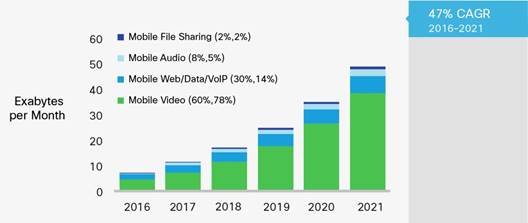
\includegraphics[width=0.5\textwidth]{mobiletraffic.jpg}
\caption{\label{fig:mobiletraffic}Mobile data forecast for 2021. Source: Cisco VNI Mobile, 2017}
\end{figure}
Alongside the growth in popularity, the user expectations on the quality of service are increasing \cite{DASH2}. To fulfill both the growth in servers load and user quality expectation, advanced technology is needed. One of these technologies is Dynamic Adaptive Streaming over HTTP (DASH), which is a protocol that has been standardized over the past eight years by MPEG, 3GPP, Open IPTV Forum, Apple, Adobe and Microsoft. \cite{HLS, MPEG, TS26.233, MS, wiki} The basic idea is to adapt dynamically the quality of the stream according to network and device conditions in order to have a smooth and seamless playback \cite{DASH1, DASH2, wiki}.
%%%%%%%%%%%%%%%%%%%%%%%%%%%%%%%%%%%
\section{Different Standards}
DASH is a MPEG protocol. In fact it is also referred to as MPEG-DASH. It is a ISO/IEC standard from 2012 (ISO/IEC 23009-1) \cite{wiki}. Latest revision is of year 2014 \cite{MPEG}. The idea is based on 3GPP Adaptive HTTP Streaming (AHS) release 9 and Open IPTV Forum release 2 \cite{wiki}. Latest 3GPP release (version 14, 2017) is maintained by the Technical Specification Group (TSG) SA4 (Services and System Aspects) and their streaming protocol is within the general name of Transparent end-to-end Packet-switched Streaming Service (PSS) (TS 26.233, TS 26.234, TS 26.244, TS 26. 247) \cite{TS26.233, TS26.234, TS26.244, TS26.247}. In particular the last one includes specifications about DASH. Apple’s HTTP Live Streaming protocol is still in draft. The first version was published in 2009 \cite{HLS} and as today it has arrived at version 23 \cite{HLS}. It doesn’t refer to the term DASH but the basic idea is still to let the client adapt the bitrate to the current network condition in order to provide a seamless playback. Another alternative of the same idea is provided by the Microsoft Smooth Streaming Protocol which first revision is of 2010 \cite{MS} and the latest is of January 2017 \cite{MS}. It is based on the Real Time Streaming Protocol (RFC 2326), which is a stateful protocol, although it makes a better use of HTTP caches and provides adaptable streaming quality through the use of MPEG-4 -based data structure \cite{MS}.
\section{The MPEG-DASH infrastructure}\label{sec:mpegdash}
All these different protocols use different names but the core structure is the same. First of all they all use HTTP as the underlying content delivery system, HTTP/1.1 in particular. We’ll talk about the advantages of using HTTP later. They all use a Media Presentation Description (which e.g. corresponds to to a Playlist in Apple's HLS \cite{HLS}) and Segments (which e.g. are called Fragments in Microsoft's SSP \cite{MS}). We present here the MPEG protocol basics.

\subsection{The data model}
MPEG-DASH \cite{MPEG} defines two basic elements and their format. The first is a Media Presentation Description (MPD) which is a XML formatted file which describes the Media Presentation, which is a bounded or unbounded list of HTTP URLs to the Segments which compose the video to be streamed. The latter is the Segment, which is the content response of an HTTP GET or partial HTTP GET (as specified in RFC 2616: HTTP/1.1 \cite{HTTP}). A Segment can contain both media data and metadata useful for segments alignment, synchronization, media navigation an other features. The client first requests the MPD and then progressively requests the Segments to be played back, until the broadcast ends or the user interrupts the process. This precess is illustrated in Figure \ref{fig:schema}. The MPD is periodically refreshed to update the list of URLs.
\begin{figure}[ht]
\centering
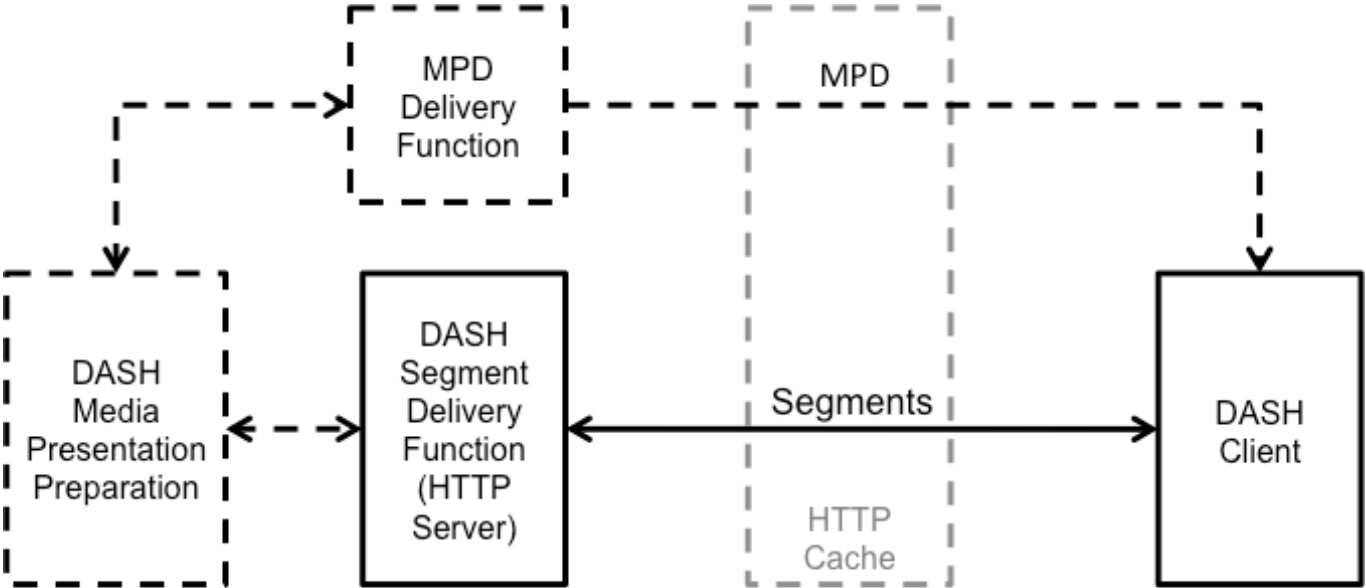
\includegraphics[width=0.5\textwidth]{DASH_schema.png}
\caption{\label{fig:schema}Streaming schema for MPEG-DASH protocol. Source: \cite{MPEG}}
\end{figure}

\par The MPD structure is illustrated in Figure \ref{fig:MPD}. 
\begin{figure}[ht]
\centering
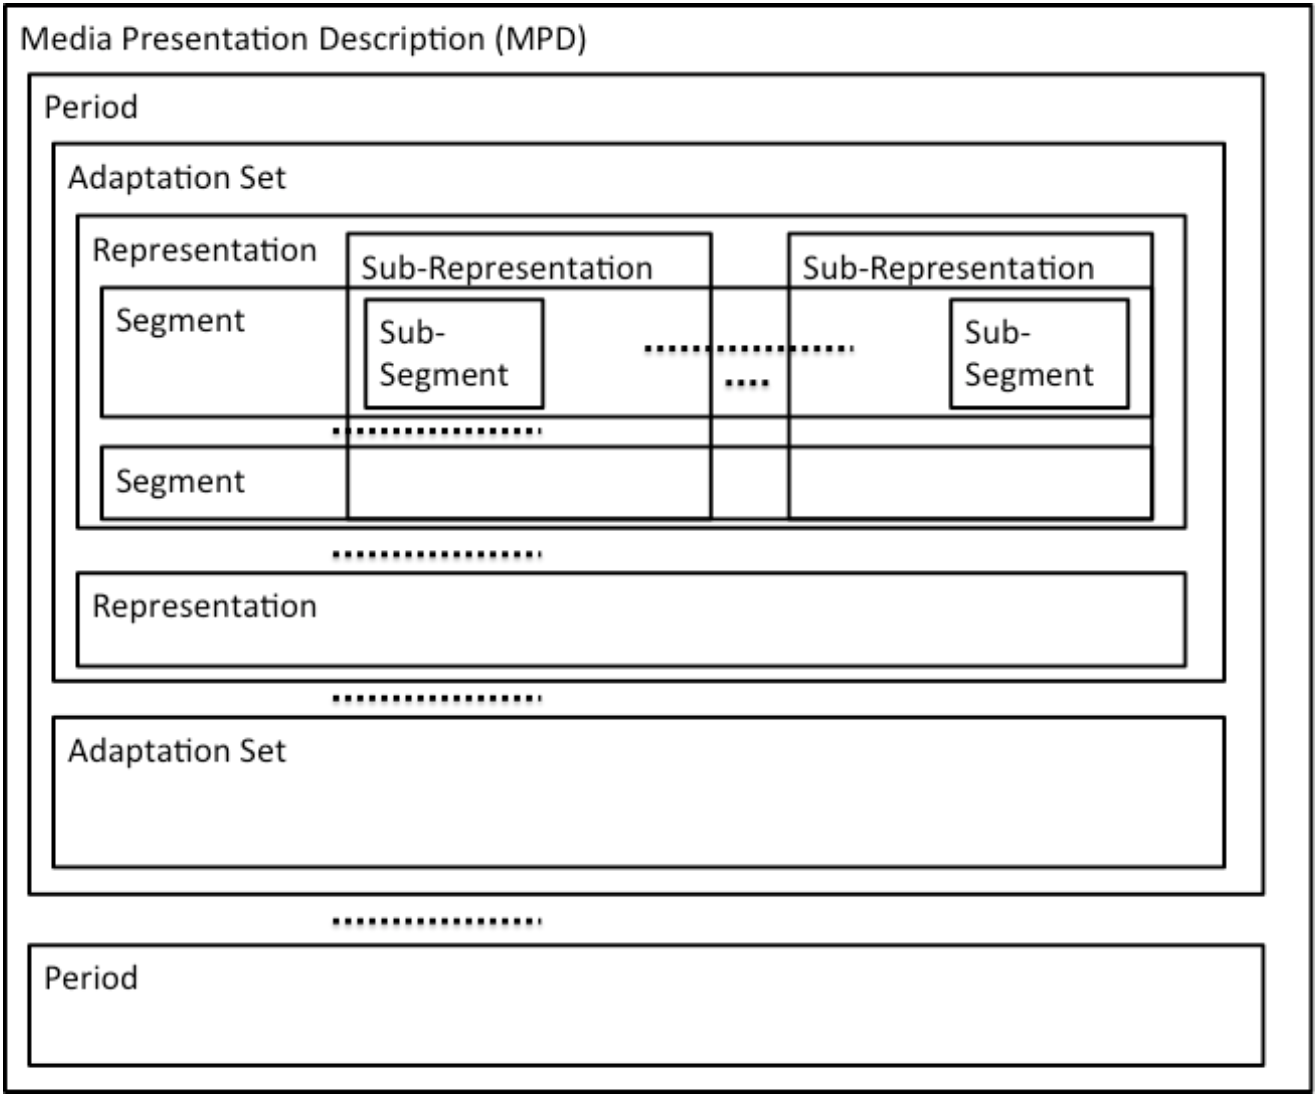
\includegraphics[width=0.5\textwidth]{MPD.png}
\caption{\label{fig:MPD}The structure of a Media Presentation Description (MPD). Source: \cite{MPEG}}
\end{figure}
In particular the MPD describes the sequence of Periods, which are media content periods during which the encoded versions of the media are consistent. The content within a period is arranged in an Adaptation Set, which contains different Representations of the media. Representations are deliverable encoded versions of one or several media content components, such as different resolutions, subtitles, languages and captions. Representations are then divided into Segments, which are the largest media units downloadable with an HTTP request, as mentioned before. Segments have more or less the same duration (which is not specified in the protocol, in contrast with Microsoft and Apple’s solutions). Periods can vary for different representations, which can be a parameter for network adaptation \cite{MPEG}, although the adaptivity is declared to be only at client side \cite{MPEG}. In particular Segment duration is a lower bound for end-to-end latency, so it is convenient to set a short Segment duration in case of low latency requirement, such us live streams \cite{MPEG}. An important feature is the possibility to divide Segments into Subsegments. This allows for Segment Indexes, which are pointers (or better byte ranges) to other Subsegments \cite{MPEG, DASH2} (Figure \ref{fig:index}). This allows the client to perform a byte range request through a partial HTTP GET request \cite{HTTP} to first download the Index, than to selectively request for specific subsegments \cite{MPEG, DASH2}. This allows for navigation through the media \cite{DASH2}. A few examples of Segment Indexing can be found in \cite{DASH2}.
\begin{figure}[ht]
\centering
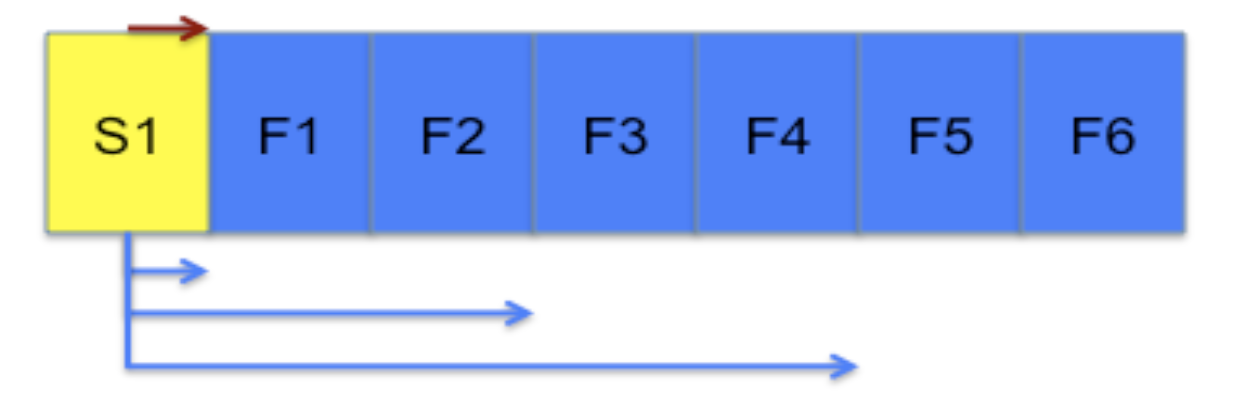
\includegraphics[width=0.5\textwidth]{index.png}
\caption{\label{fig:index}Index and media Subsegments. An Index Subsegment points to the first media Subsegment and to other Subsegments. Source: \cite{DASH2}}
\end{figure}
Clients may decide to jump from one representation to another. This is made easier through Stream Access Points, usually located at the beginning of Segments or Subsegments, where the different Representations are aligned, in order to play back subsequent media segments with continuous timestamps, without audio or video glitches and without downloading overlapping media content \cite{MPEG, DASH2}.

\subsection{The DASH client model}
MPEG-DASH \cite{MPEG} considers a DASH client model logically composed of three parts, as shown in Figure \ref{fig:client}. The first part is the DASH access engine, which can request and receive the Media Presentation Description and the Segments (or part of them) from an HTTP server and handle them as described in the protocol. It then passes to the Media engine module the media in MPEG format plus timing information that maps the media internal timestamps to the presentation timestamps. The access engine also receives and extracts Events which can be handled by the access engine itself or handed off to a different Application module.
\begin{figure}[ht]
\centering
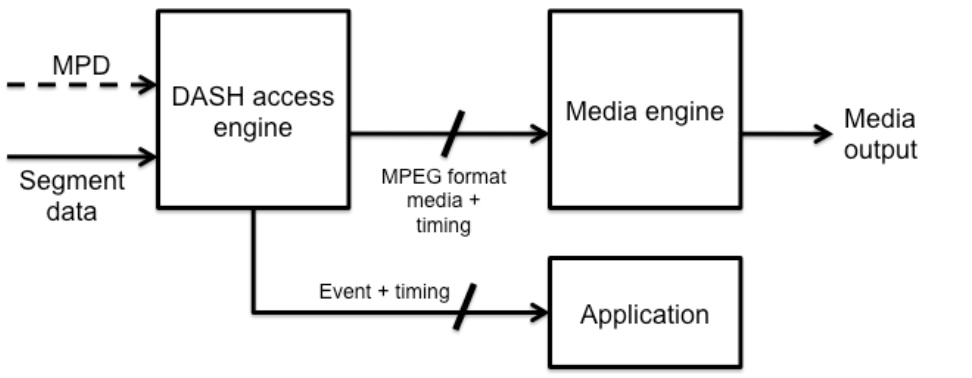
\includegraphics[width=0.5\textwidth]{Client.png}
\caption{\label{fig:client}MPEG-DASH Client Model: \cite{MPEG}}
\end{figure}

\section{Why HTTP is a good idea}
The main solution for streaming before DASH was widely adopted was the Real Time Streaming Protocol. It was a stateful protocol in which the client established a connection with a server and the latter kept the state of the client, sending it a continuous stream of packets through UDP or TCP until it disconnected \cite{DASH2}. HTTP is a stateless protocol in which requests and responses of some data are considered as a complete stand-alone transaction, as shown in Figure \ref{fig:http}.
\begin{figure}[ht]
\centering
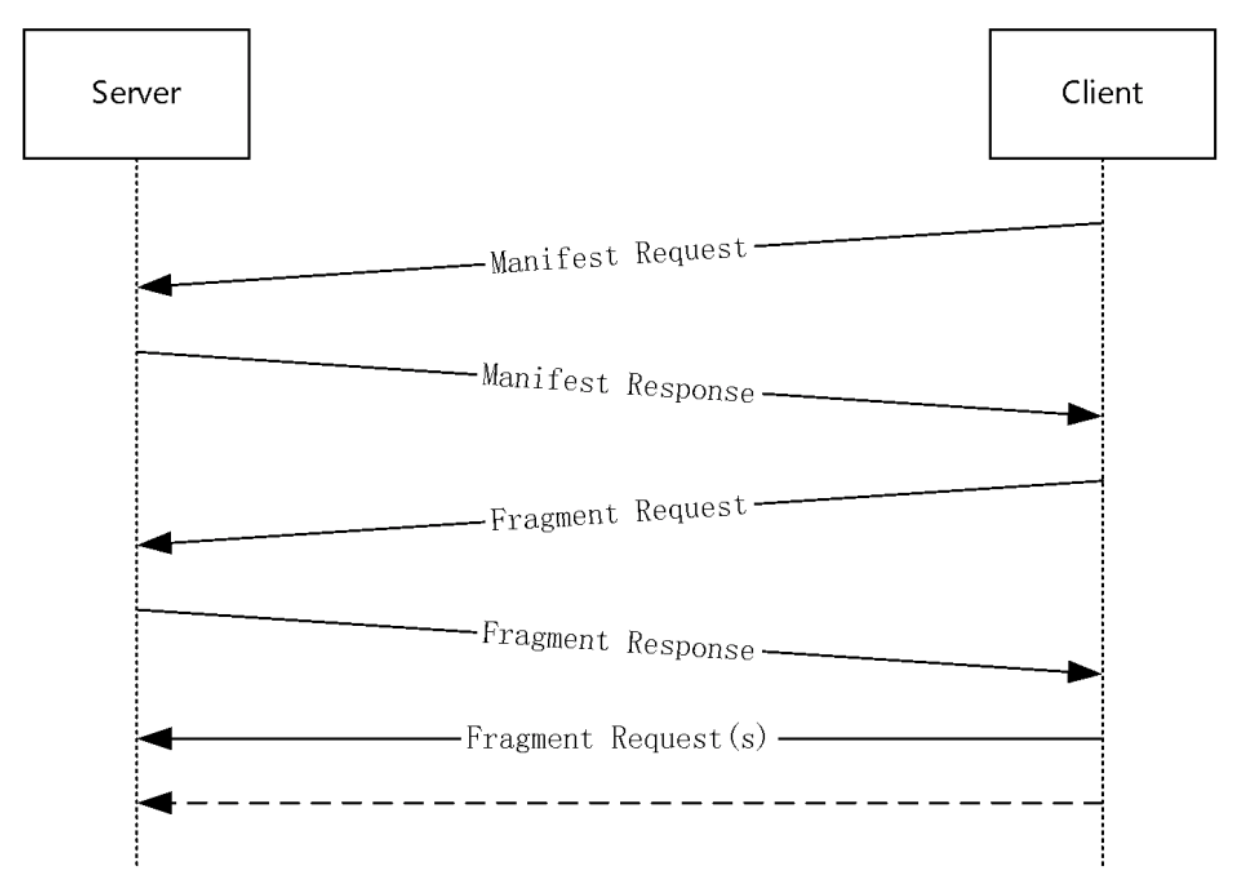
\includegraphics[width=0.5\textwidth]{http.png}
\caption{\label{fig:http}Communication between client and server in the DASH protocol through HTTP. Source: \cite{MS}}
\end{figure}
Through HTTP the streaming session is completely handled by the client, avoiding an overhead from the frequent communication between the client and the server to maintain a stateful connection (only one or more simple TCP connection are held) \cite{DASH2, HTTP}. Another alternative is HTTP progressive download through byte ranges requests \cite{DASH2}. The disadvantages of this are that the whole content must be ready in advance, therefore it isn't suitable for live streaming. Moreover bandwidth might be wasted if the user decides to stop watching the stream. Last and most important, it isn't bitrate adaptive \cite{DASH2}. For these reasons HTTP progressive download wasn't enough for the new streaming technologies requirements. However the preexisting Content Delivery Networks based on HTTP were widely developed and efficient and could be exploited. An example of a general media distribution architecture is in Figure \ref{fig:architecture})
\begin{figure}[ht]
\centering
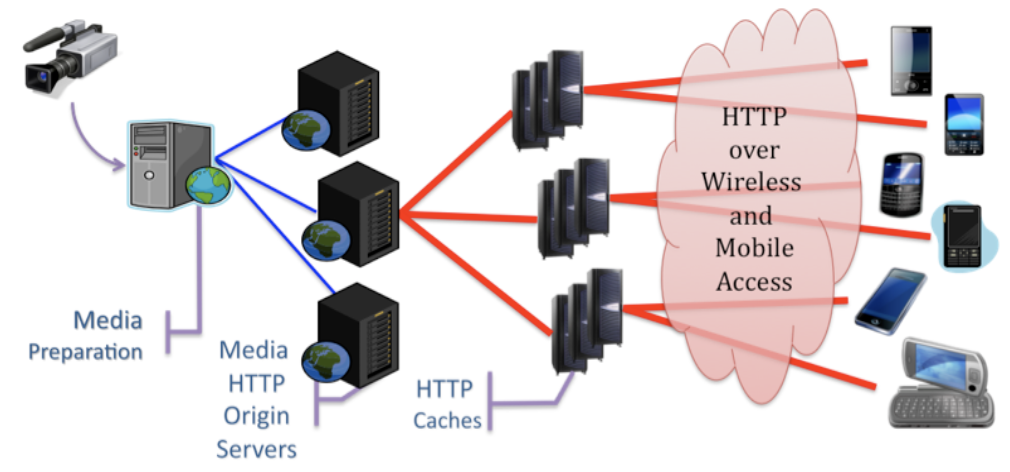
\includegraphics[width=0.5\textwidth]{architecture.png}
\caption{\label{fig:architecture}HTTP media distribution architecture with HTTP caches. Source: \cite{DASH2}}
\end{figure}, where a video is taken from a source and a Media Preparation server encodes it with different bitrates, than splits the different versions into segments according to the protocol. Than the segments are sent with the Media Presentation Description to several HTTP Servers. The client requests the segments according to some adaptation algorithm, taking in consideration various elements such as network condition, available bandwidth, device conditions or user preferences. The HTTP response can be speeded-up thanks to HTTP cache servers, as illustrated in Figure \ref{fig:caching} \cite{DASH1, DASH2, MS}.
\begin{figure}[ht]
\centering
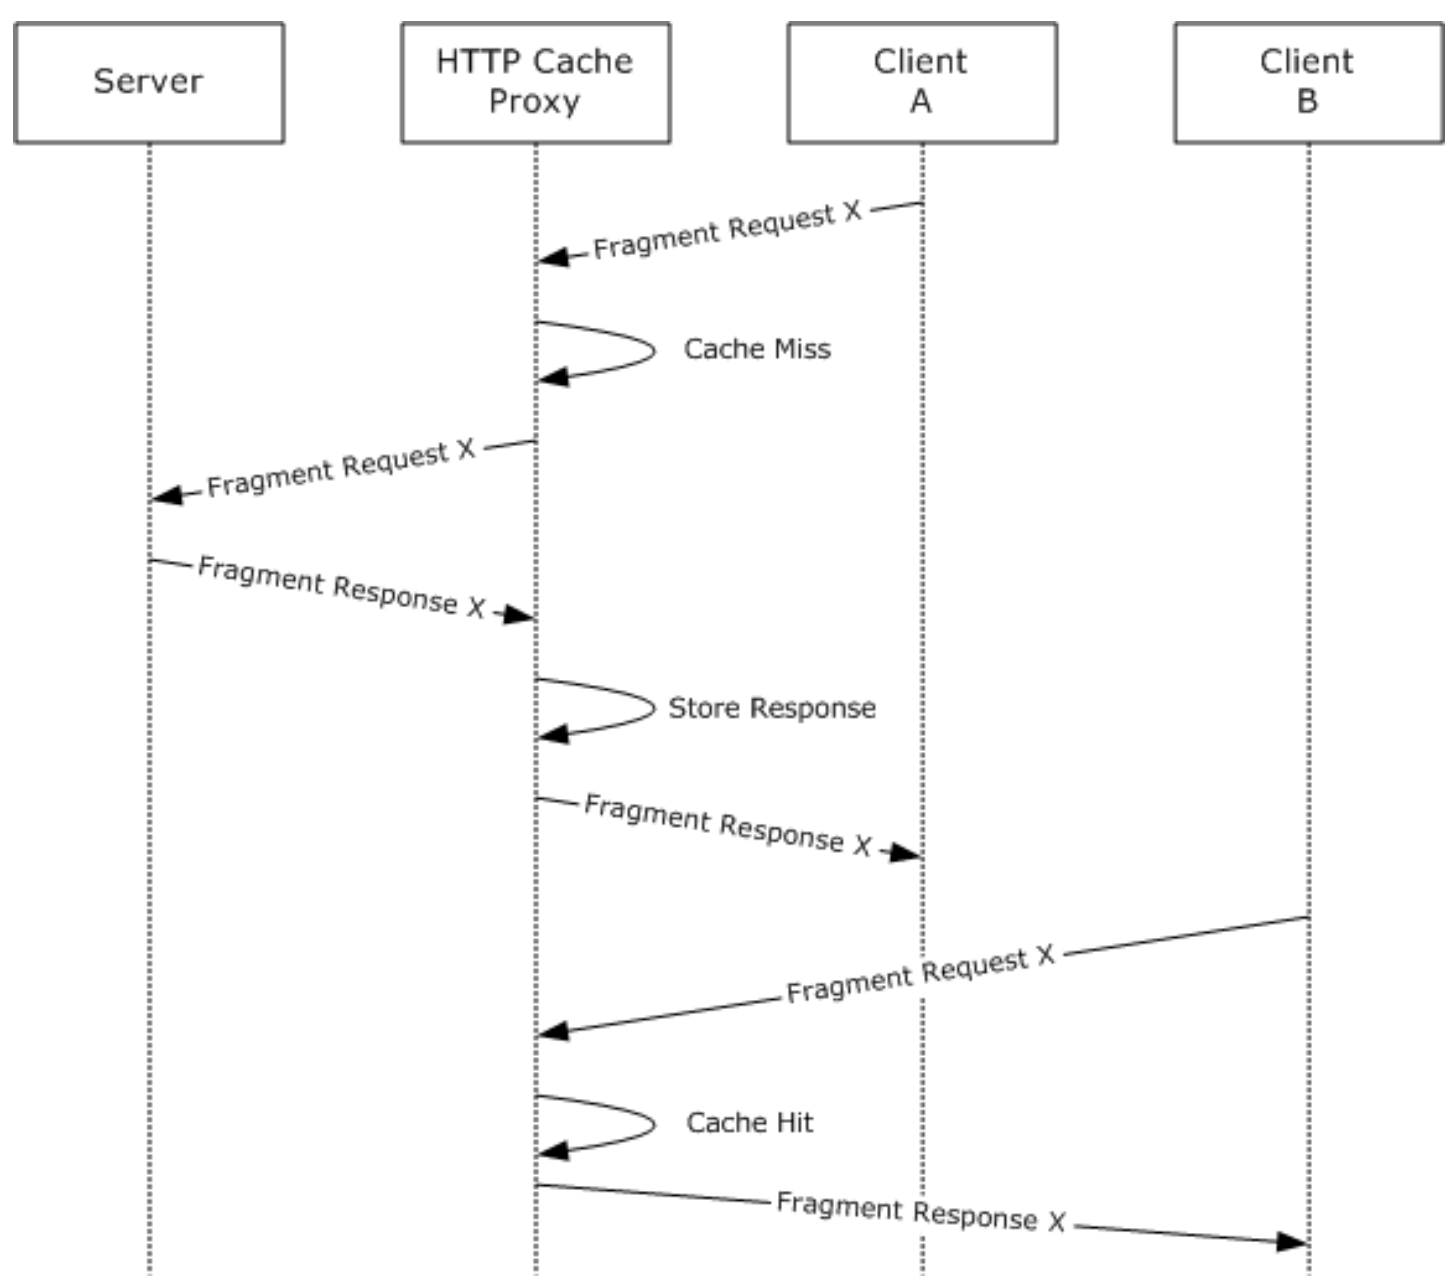
\includegraphics[width=0.5\textwidth]{caching.png}
\caption{\label{fig:caching}Efficient content delivery with the use of HTTP caches. Source: \cite{MS}}
\end{figure}
Not only the HTTP transaction is quicker with CDNs but the massive amount of connections to be handled are offloaded from the central servers and distributed to the peripheral servers. For these advantages provided by HTTP CDNs, they were chosen as a base for Dynamic Adaptive Streaming \cite{DASH2}. 
Another reason for choosing HTTP is that it is the most used protocol for content delivery and communication over World Wide Web and so the user doesn't need to have particular skills to set up the firewall properly in order to receive the stream, since most firewalls let the traffic pass through the standard HTTP port \cite{DASH1, DASH2}. 
Other advantages of using HTTP are that the client can decide the initial streaming quality based on the currant bandwidth without having to negotiate with the server \cite{DASH2} (stateless  connection), as well as the ability to decide to switch stream quality independently from the server \cite{DASH2}.



\section{Adaptive Bit Rate algorithms}\label{sec:abr}
% general introduction on ABR algorithms and brief description of the section 
In this section we describe some algorithms that can be used to adapt the bit rate in order to better exploit the available bandwidth.

In general, these algorithms are called Adaptive Bit Rate (ABR) algorithms, and they are designed with three goals in mind \cite{ABR}:
\begin{enumerate}
\item maximize efficiency: stream at the highest possible bit rate;
\item minimize re-buffering: avoid playback freezing;
\item stability: switch bit rate only when necessary.
\end{enumerate}
The first goal is meant to serve the user with the best video quality possible: to meet this requirement, the client will choose the highest bit rate that the bandwidth, in conjunction with the buffer, can sustain. However the channel is not the only criterion by which the client will choose the bit rate: also the screen size of the device, the size of the player video and the CPU come into play in order to avoid waste of resources. The second and the third goal are meant to offer the user the best experience possible: fast start-up time, avoid playback freezing events and refrain to switch bit rate if it is not strictly required in order to provide smooth streaming \cite{QoEDASH}.

In literature we can find many algorithms and implementations that work either on the client side or on the server side. We here focus our attention on the former and we see two of them.

\subsection{Segment Aware Rate Adaptation}\label{subsec:sara}
Segment Aware Rate Adaptation (SARA) is an ABR algorithm that decides the bit rate to be selected for each segment of the video depending not only on the current network condition and the buffer occupancy but also on the size of the segment to be downloaded. 

As described in section \ref{sec:mpegdash}, each video is encoded with different selection of resolutions and bit rates and then it is divided in multiple segments. The server collects all this information in the MPD file. Since each segment is usually of a fixed playback duration but differs greatly on size (see figure \ref{fig:segnumb}), some algorithms proposed in literature may fail to predict the time to download the next segment \cite{SARA}. SARA instead proposes to enhance the MPD file with the size of each segment and then estimates the throughput based also on this information.

\begin{figure}[ht]
\centering
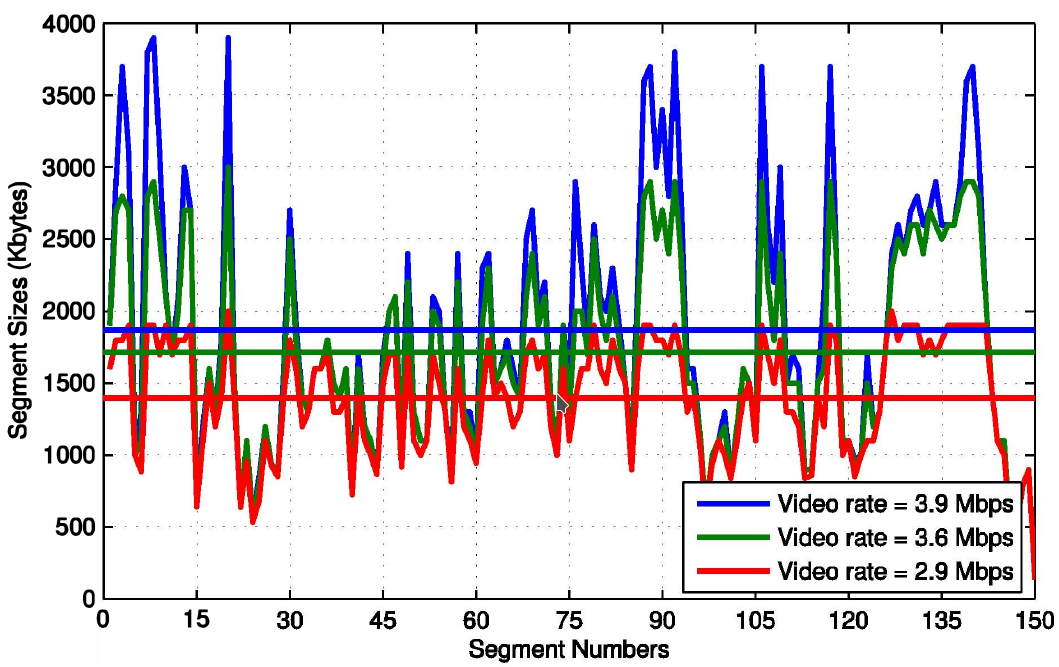
\includegraphics[width=0.5\textwidth]{sara_segment_numbers}
\caption{Variation in segment sizes for \textit{The Big Buck Bunny Movie }\cite{BBB}. Each segment lasts for 4 seconds and it is encoded with three different bit rates. Source: \cite{SARA}}\label{fig:segnumb}
\end{figure}

In order for the rate adaptation algorithm to pick the appropriate bit rate, it is necessary to measure the throughput during the entire video session: to avoid the effect of instantaneous throughput variation we use harmonic mean \cite{SARA}. For a generic segment $i$ we assign a weight $w_i$ that is proportional to the segment size. Then, we take into account the download rates of the segments, call them $d_1, d_2, \cdots$. The weighted harmonic mean download rate for $n$ downloaded segments is then
\[
H_n=\frac{\sum_{i=1}^n w_i}{\sum_{i=1}^n \frac{w_i}{d_i}}
\]
Based on this value, we can predict the time to download the next segment as $w_{n+1}/H_n$.

So, from the set of all representations, SARA selects to download the most suitable one. Every segment that is downloaded is stored on a buffer $B$. This buffer have a maximum capacity $B_{max}$, a current capacity $B_{curr}$ and three other thresholds $I$, $B_{\alpha}$ and $B_{\beta}$. The buffer is pictured in \ref{fig:sarabuffer} and all of the thresholds are defined in terms of the number of segments.

\begin{figure}[ht]
\centering
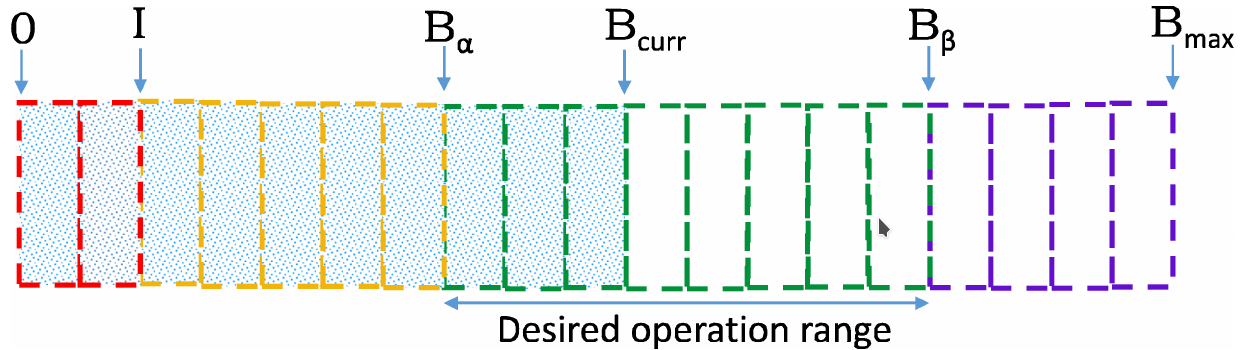
\includegraphics[width=0.5\textwidth]{sara_buffer_thresholds}
\caption{Buffer and the thresholds. Source: \cite{SARA}}\label{fig:sarabuffer}
\end{figure}

The algorithm works based on the current buffer capacity and the predicted next segment download time. It works in four stages:
\begin{itemize}
\item \textbf{Fast Start} ($B_{curr} \leq I$): the algorithm selects the lowest bit rate. This ensure that the start up time of the playback is kept as small as possible. This is important to prevent the user to abandon the video session \cite{QoEDASH}.
\item \textbf{Additive Increase} ($ I < B_{curr} \leq B_{\alpha}$): in this stage we start to increase the bit rate. This is done in small steps to avoid the buffer to go back under $I$.
\item \textbf{Aggressive Switching} ($ B_{\alpha} < B_{curr} \leq B_{\beta}$): now, based on the network condition and the buffer occupancy, we start to select the most suitable bit rate that is greater than or equal to the current one. 
\item \textbf{Delayed Download} ($B_{\beta} < B_{curr} \leq B_{max}$): in this stage, the most suitable bit rate for the current network condition is selected, however the request is delayed until the buffer occupancy goes under $B_{\beta}$. This ensures two things: it prevents buffer overflows and it avoids unnecessary downloads of segments in case the user stops the playback. 
\end{itemize}

The algorithm is listed in \ref{alg:sara}. The algorithm is called after every segment downloaded to determine the representation to download for the next segment.

At the start of the video session or after a re-buffering event, the number of segments in the buffer is below $I$ and so the algorithm works in the \textit{Fast Start} phase: the lowest bit rate is selected. When the capacity of the buffer is beyond $I$, the algorithm switches to the \textit{Additive Increase} phase.

The time required to download the next segment is given by $w_{n+1}^{curr}/H_n$. In general, any time during the playback of the video, if the download time of the next segment is greater than $B_{curr}-I$, it is not feasible to download the next segment of the current bit rate before the buffer goes below $I$: the best possible bit rate is chosen among the ones that can be downloaded in the duration $B_{curr}-I$, given the next segment size and the current weighted Harmonic mean download rate. SARA uses a conservative approach and tries to keep the buffer above the $I$ threshold; if it is not possible, it switches to the lowest bit rate possible.

In the \textit{Additive Increase} phase the algorithm starts increasing the bit rate of the video, if possible. The increase in quality is done step by step: if the current representation has a bit rate $r^{curr}$, the next one will have a bit rate that is the minimum bit rate, among the ones available, that is greater than $r^{curr}$. This approach ensures that the quality is increased gradually.

After the buffer capacity goes above $B_{\alpha}$ the increase in quality is more aggressive and the algorithm selects the representation with the highest bit rate that can be downloaded before the buffer capacity goes under $I$. During the \textit{Aggressive Switching} phase, the request is sent immediately, but when it enter the \textit{Delayed Download} phase ($B_{curr} > B_{\beta}$), the request is sent only when the buffer goes below $B_{\beta}$, thus avoiding buffer overflows or unnecessary data fetch in case the user stops the video session prematurely.

\begin{algorithm}[H]
 \caption{Segment Aware Rate Adaptation algorithm}\label{alg:sara}
 \begin{algorithmic}[1]
 \renewcommand{\algorithmicrequire}{\textbf{Input:}}
 \renewcommand{\algorithmicensure}{\textbf{Output:}}
 \REQUIRE $\mathfrak{R}$: set of the available bit rates $\{r^{min}, \cdots, r^i ,\cdots, r^{max}\}$
 \\ $I$, $B_{\alpha}$, $B_{\beta}$: buffer thresholds (constants) 
 \\ $n$: segment number of the most recent download 
 \\ $r^{curr}$: bit rate of the most recent downloaded segment
 \\ $B_{curr}$: current buffer occupancy in seconds
 \\ $W_{n+1}=\{w_{n+1}^{min},\cdots, w_{n+1}^{i},\cdots, w_{n+1}^{max}\}$ the sizes of the segments of bit rate $\{r^{min}, \cdots, r^i ,\cdots, r^{max}\}$
 \\ $H_n$: weighted Harmonic mean download rate for the first $n$ segments
 \ENSURE  $l_{n+1}$: the bit rate of the next segment to be downloaded
 \\ $\delta$: the wait time before download the next segment
 
 \IF{$B_{curr} \leq I$}
 	\STATE $l_{n+1} = r^{min}$;
 \ELSE
 	\IF{$\frac{w_{n+1}^{curr}}{H_n} > B_{curr} - I$}
    	\STATE $l_{n+1} = \max\{r^i\ |\ r^i\in\mathfrak{R},\ \frac{w_{n+1}^{i}}{H_n} \leq B_{curr} - I,\ i \leq curr \}$;
        \STATE $\delta = 0$;
     \ELSIF{$B_{curr}\leq B_{\alpha}$}
     	\IF{$\frac{w_{n+1}^{curr+1}}{H_n} < B_{curr} - I$}
        	\STATE $l_{n+1} = \min\{r^i\ |\ r^i\in\mathfrak{R},\ r^i > r^{curr},\  i \geq curr \}$;
        \ELSE
        	\STATE $l_{n+1} = r^{curr}$;
        \ENDIF
    	\STATE $\delta = 0$;
    \ELSIF{$B_{curr}\leq B_{\beta}$}
    	\STATE $l_{n+1} = \max\{r^i\ |\ r^i\in\mathfrak{R},\ \frac{w_{n+1}^{i}}{H_n} \leq B_{curr} - I,\ i \geq curr \}$;
        \STATE $\delta = 0$;
      \ELSIF{$B_{curr} > B_{\beta}$}
      	\STATE $l_{n+1} = \max\{r^i\ |\ r^i\in\mathfrak{R},\ \frac{w_{n+1}^{i}}{H_n} \leq B_{curr} - B_{\alpha},\ i \geq curr \}$;
        \STATE $\delta = B_{curr} - B_{\beta}$;
      \ELSE
      	\STATE $l_{n+1} = r^{curr}$;
        \STATE $\delta = 0$;
    \ENDIF
 \ENDIF
 \end{algorithmic}
\end{algorithm}

\paragraph*{Performance} How well does SARA perform? In \cite{SARA} the proposed algorithm is compared with a very basic adaptive algorithm: it uses the average segment download rate and the current buffer occupancy to select the next segment. It starts downloading the video at the lowest possible bit rate and it measures the average download rate. When the buffer capacity is beyond $I$ (same as in SARA), the algorithm, based on the average download rate and the buffer capacity, chooses the next segment as the one with the bit rate closest to the available bandwidth. The switching-up and switching-down is optimistic.

The basic algorithms is set with $I=2$ and $B_{max}=10$. The SARA algorithm is set with $I=2$, $B_{\alpha}=5$, $B_{\beta}=10$ and $B_{max}=12$.

\begin{figure}[ht]
\centering
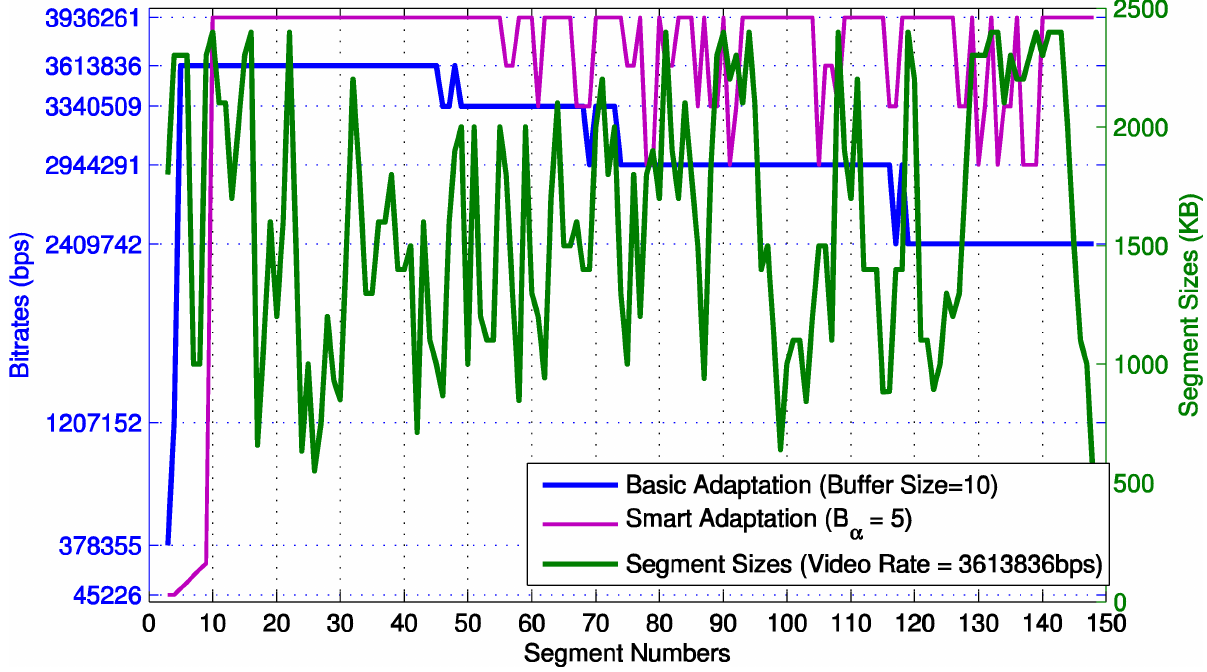
\includegraphics[width=0.5\textwidth]{sara_basic_segment}
\caption{Effect of segment sizes on Basic and SARA with a bandwidth of 1 Mbps. Source: \cite{SARA}}\label{fig:sarabasicseg}
\end{figure}

In figure \ref{fig:sarabasicseg} is depicted the variation of the bit rate chosen by both algorithms. Even with a steady bandwidth, SARA performs better than the basic algorithm: the great variation of segment sizes affected both algorithm but since SARA knew before hand the segment sizes it could anticipate their decreasing, thus choosing a better bit rate. 

\begin{figure}[ht!]
\centering
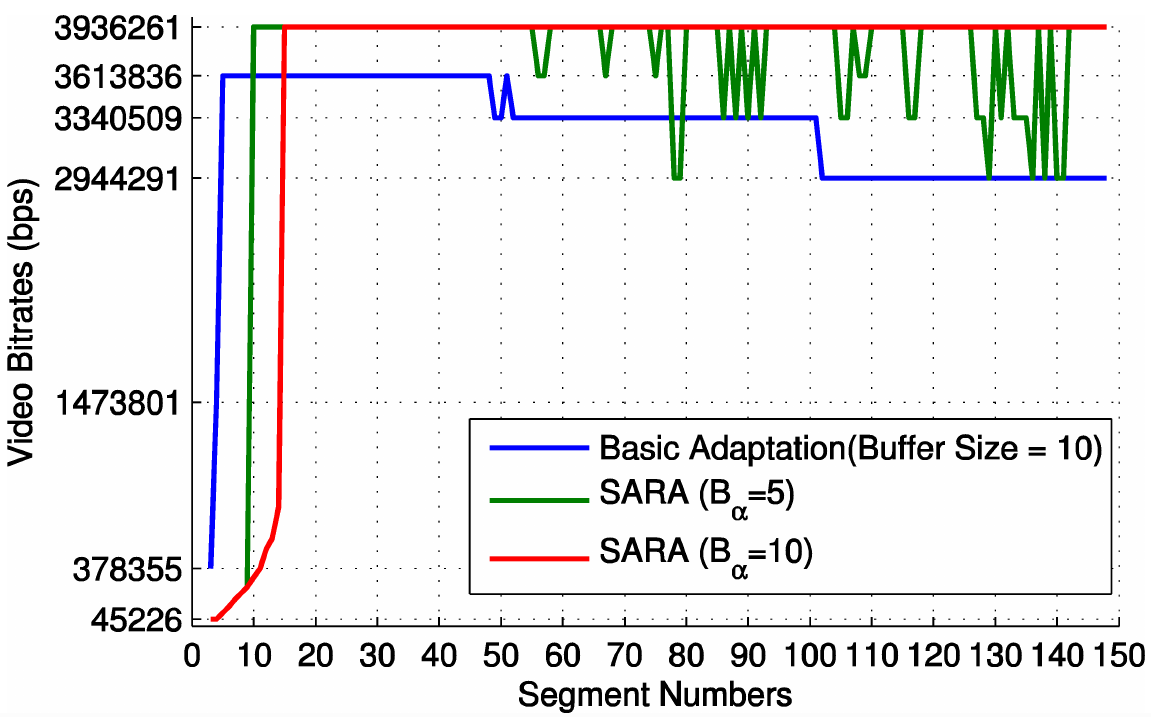
\includegraphics[width=0.5\textwidth]{sara_basic_4m}
\caption{Bit rate variation with bandwidth of 4 Mbps. Source: \cite{SARA}}\label{fig:sarabasic4m}
\end{figure}

\begin{figure}[ht!]
\centering
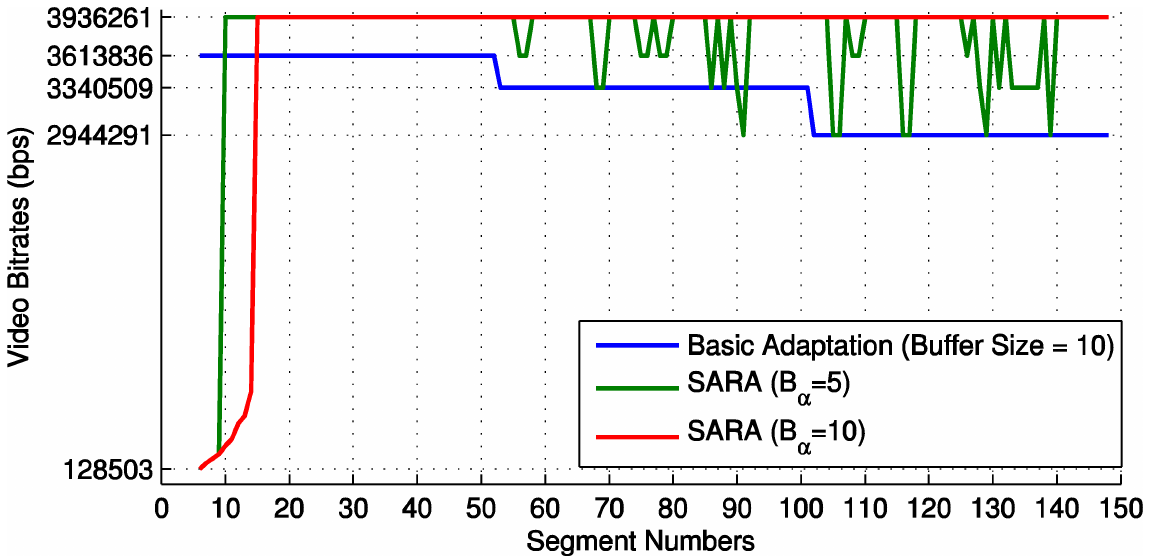
\includegraphics[width=0.5\textwidth]{sara_basic_8m}
\caption{Bit rate variation with bandwidth of 8 Mbps. Source: \cite{SARA}}\label{fig:sarabasic8m}
\end{figure}

In figures \ref{fig:sarabasic4m} and \ref{fig:sarabasic8m}, we see that SARA keeps performing better than the basic algorithm even when the available bandwidth is greater. Overall SARA chooses a better bit rate and the buffer avoids SARA to switch-down the bit rate in response to a sudden decrease of the segment sizes.

\subsection{Buffer-based Bit Rate Adaptation}\label{subsec:buffer}
In this section we illustrate a buffer based adaptation algorithm, that is an algorithm that decides the bit rate mainly based on the buffer characteristics.

If the throughput drops suddenly, requesting video segments with an increase in quality may lead to a buffer underflow, thus interrupting the playback. With the algorithm proposed in \cite{buffer}, we try to estimate the buffer level in the near future to avoid buffer underflows.

First, we provide two definitions:
\begin{itemize}
\item \textbf{Arrival curve}: represents the accumulated data size received by the client at a given time $t$;
\item \textbf{Playback curve}: represents the accumulated data size consumed by the client at a given time $t$.
\end{itemize}
An example of these curves is plotted in picture \ref{fig:buffercurves}. Suppose that the client starts receiving data at time $t_0^r$ and the playback starts at time $t_0^p$: then, the initial buffering data is $(t_0^r-t_0^p)$ seconds. If the average arrival rate is equal to the playback rate, the buffer will be stable.

\begin{figure}[ht]
\centering
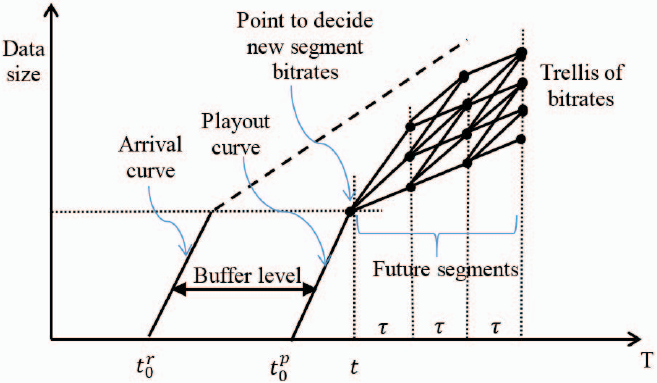
\includegraphics[width=0.5\textwidth]{buffer_curves}
\caption{Arrival curve and playback curve. Source: \cite{buffer}}\label{fig:buffercurves}
\end{figure}

In the following, suppose that the server has a set of $K$ representations for each segment: the set of possible bit rates is $\mathfrak{R}=\{R_0, R_1, \cdots, R_{K-1}\}$. With $B_l$ we denote the request bit rate for segment $l$. At time $t_i$, after downloading the current segment $i$ with bit rate $B_i$, the client decides a sequence of bit rates for the next $N$ segments $\{b_{(i,1)}, b_{(i,2)}, \cdots, b_{(i,N)}\}$, where $(i,j)$ means the segment $i+j$ and $b_{(i,j)}$ means the bit rate decided for the segment $i+j$. This sequence of bit rates is called a path $P$.

In picture \ref{fig:buffercurves} we see trellis of bit rates: those are all the possible sequences of bit rates that the client could decide to request at time $t$. Thus, the decision problem is represented by a trellis in which each sequence of bit rates is shown as a path. 

We observe that the video bit rate $b_{(i,0)}=B_i$ is the video bit rate requested for the current segment and it is considered as the starting point of our path $P$. Moreover, the final bit rate $b_{(i,N)}$ in path $P$ should be the highest value but lower than the current throughput $T_{curr}$, that is $b_{(i,N)} = \sup\{R_k\in\mathfrak{R}\ :\ R_k<T_{curr}\}$, because the client has to preserve its buffer. 

At each step, we denote with $\beta_{(i,j)}$, $0\leq\beta_{(i,j)}\leq\beta_{max)}$ and $\beta_{max}$ the maximum buffer size, the buffer level right after downloading the segment $(i,j)$. An estimation of the buffer level could be the following:
\begin{equation}\label{eq:beta}
\beta_{(i,j)}=\begin{cases}
\beta_{(i,j-1)} + \tau\cdot\left(1-\frac{b_{(i,j)}}{T_{(i,j}}\right)\ \ \ &\forall j>0 \\
\beta{(i,0)} \ \ \ \ &j=0
\end{cases}
\end{equation}
where $\tau$ is the duration of the segment $(i,j)$, $T_{(i,j)}$ is the estimated throughput for segment $(i,j)$, thus the interval to download segment $(i,j)$ is $\frac{\tau\cdot b_{(i,j)}}{T_{(i,j)}}$. To avoid buffer underflows, all estimations of the buffer level need to be higher than a predefined minimum $\beta_{min}$, that is
\begin{equation}\label{eq:betamin}
\beta_{(i,j)} \geq \beta_{min},\ \ \ 1\leq j\leq N
\end{equation}
needs to hold.

Now, we assume the in the near future the throughput remains close to the estimated throughput $T_{est}\cong T_{(i,N)}\cong T_{(i,N-1)}\cong \cdots \cong T_{(i,0)}$. Then, equation \ref{eq:beta} becomes
\begin{equation}\label{eq:betaest}
\beta_{(i,j)}=\begin{cases}
\beta_{(i,j-1)} + \tau\cdot\left(1-\frac{b_{(i,j)}}{T_{est}}\right)\ \ \ &\forall j>0 \\
\beta{(i,0)} \ \ \ \ &j=0
\end{cases}
\end{equation}
Using the throughput estimation of \cite{throughputest}, where the throughput estimate is stable under small fluctuations but highly responsive on sudden changes of bandwidth, after the client has decided a path $P$ at time $t_i$, it builds a new path $P'$ at time $t_{i^'}$ only if the throughput has changed by an arbitrary factor.

\begin{algorithm}[H]
 \caption{Bit rate selection for segment $(i,j)$}\label{alg:bufferalg}
 \begin{algorithmic}[1]
 \renewcommand{\algorithmicrequire}{\textbf{Input:}}
 \renewcommand{\algorithmicensure}{\textbf{Output:}}
 \REQUIRE $j$, $b_{(i,j-1)}$, $\beta_{(i,j-1)}$
 \ENSURE  $b_{(i,j)}$, $\beta_{(i,j)}$
 \FOR{$b_{(i,j)} := (b_{(i,j-1)} + \Delta b) \rightarrow b_{(i,N)}$}
 	\STATE $\beta_{(i,j-1)} + \tau\cdot\left(1-\frac{b_{(i,j)}}{T_{est}}\right)$
    \IF{$\beta_{min} < \beta_{(i,j)}$}
    	\IF{$b_{(i,j)}=b_{(i,N)}$}
        	\STATE $P := \{b_{(i,0)}, b_{(i,1)}, \cdots , b_{(i,j)}\}$;
            \STATE ** store path $P$ and stop **;
        \ELSIF{$j<N$}
        	\STATE ** select bit rate for segment $(i,j+1)$ with input parameters
            $(j+1, b_{(i,j)}, \beta_{(i,j)})$ **
        \ENDIF
    \ENDIF
 \ENDFOR
 \end{algorithmic}
\end{algorithm}

The algorithm \ref{alg:bufferalg} describes how the path is built. Since the client will request the final segment after $N$ segments, the simplest way to build the path is to request video bit rates with a small change per step. This amount should be
\begin{equation*}
\Delta b = \frac{b_{(i,N)} - b_{(i,0)}}{N};
\end{equation*}
in this way we keep the standard deviation of the decided bit rates in path $P$ small \cite{buffer}. From the user perspective this means that the video quality changes gradually, thus providing a smooth playback.

The buffer estimation is done by applying equation \ref{eq:betaest} and, to avoid buffer underflows when there is a drastically degradation of the throughput, constraint \ref{eq:betamin} is enforced. Note that this algorithm works also in the case the throughput increases: this time, $\Delta b>0$, \ref{eq:betamin} keeps holding and the path is decided with small increasing steps.  

The last step is to decide $N$. If the current buffer level is high, then $N$ can be set to a high value: the client decides the video bit rates with smaller steps and need a larger number of segments to reach the final bit rate. On the contrary, if the current level of the buffer is small, it is better to set $N$ at a low value in order to react quickly to the throughput change. Then $N$ could be set as follows
\begin{equation*}
N = \left[R_{buffer}\cdot\Omega + 1\right]
\end{equation*}
where $R_{buffer}$ is the buffer ratio function, defined as
\begin{equation*}
R_{buffer}=\begin{cases}
\frac{\beta_{curr} - \beta_{min}}{\beta_{max} - \beta_{min}}\ \ \  &\beta_{curr} > \beta_{min} \\
0 &\beta_{curr}\leq\beta_{min}
\end{cases},
\end{equation*}
and $\Omega$ is a constant that represent the aggressiveness of path $P$. Note that in the worst case ($\beta_{curr}\leq\beta_{min}$), the algorithm behaves exactly as the instant throughput based method.

\subparagraph*{Performance} In the following we show some experimental results of the proposed algorithm. The various constants described in the previous paragraph are set as follows: $\beta_{min}=\beta_{max}/2=10$ seconds, $\Omega = 6$ and the path is built every time the throughput estimation changes by at least $10\%$. 

The proposed algorithm is compared with two other algorithms. The first one, here called "Aggressive method", is an instant throughput based algorithm, that is, the client selects the representation of the next segment to download only based on the instant throughput of the last segment downloaded \cite{buffercomparison}. The second one, here called "Threshold-based method", is a different buffer based method: it defines three thresholds on the buffer capacity, $0\leq B_{min} < B_{low} < B_{max}$, and it chooses the next segment to download based on how much data are stored in the buffer. If the buffer capacity is in the interval $[0, B_{min})$, it starts downloading the next segment with the lowest bit rate in order to ensure that the playback of the video starts as soon as possible and subsequently, if the throughput is high enough, it switches to a higher representation. When the buffer capacity is greater or equal to $B_{min}$, the aggressiveness of the algorithm increases. The goal is to keep the buffer capacity in the interval $[B_{low}, B_{max}]$ \cite{buffercomparison}. The thresholds are set as follows: $B_{min}=5 s$, $B_{low}=10 s$, $B_{max}=20 s$ \cite{buffer}.

\begin{figure}[ht!]
	\centering
	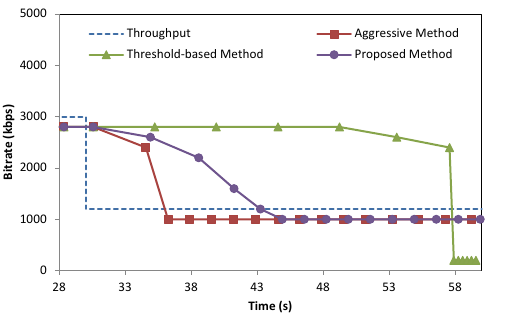
\includegraphics[width=0.5\textwidth]{buffer_bitrate_low}
    \caption{Adapted bit rate on a simple scenario. Source: \cite{buffer}}\label{fig:bufferbitratesimple}
\end{figure}

\begin{figure}[ht!]
	\centering
	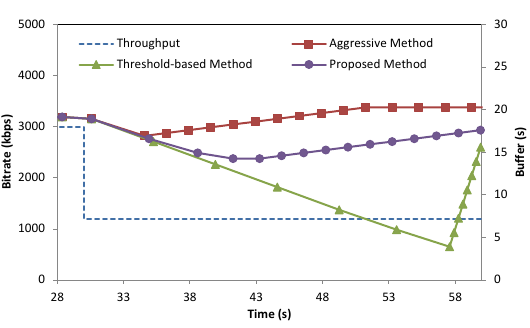
\includegraphics[width=0.5\textwidth]{buffer_buffer_capacity}
    \caption{Buffer capacity on a simple scenario. Source: \cite{buffer}}\label{fig:buffercapacitysimple}
\end{figure}

In figures \ref{fig:bufferbitratesimple} and \ref{fig:buffercapacitysimple} we can see the adapted bit rate and the buffer capacity on a simple scenario. The "Aggressive method" reacts quickly to the change in throughput, however the bit rate variations could impact negatively to the user experience since it cannot select representation above the throughput even when the buffer is full. The "Threshold-based method" instead tries to keep the bit rate high but when the buffer level goes below the minimum it switches to the lowest representation in order to keep the buffer in the target interval. The algorithm proposed here selects the representation with a gradually decreasing bit rate (small steps of $400$ kbps \cite{buffer}) and the buffer level is maintained and rarely goes below the minimum.

\begin{figure}[ht!]
	\centering
	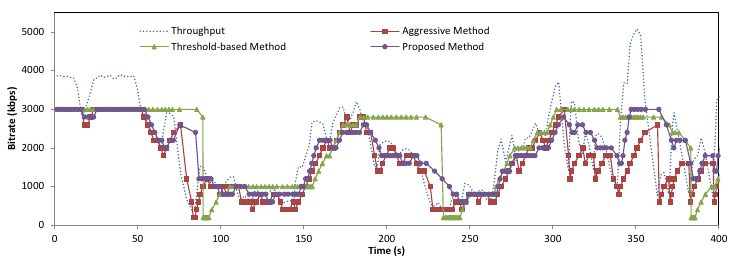
\includegraphics[width=0.5\textwidth]{buffer_bitrate_normal}
    \caption{Adapted bit rate on a complex scenario. Source: \cite{buffer}}\label{fig:bufferbitratecomplex}
\end{figure}

\begin{figure}[ht!]
	\centering
	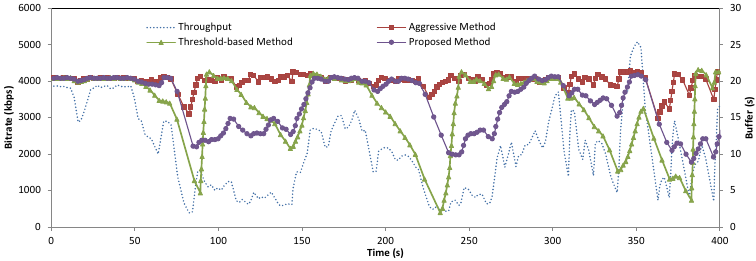
\includegraphics[width=0.5\textwidth]{buffer_buffer_normal}
    \caption{Buffer capacity on a complex scenario. Source: \cite{buffer}}\label{fig:buffercapacitycomplex}
\end{figure}

In figures \ref{fig:bufferbitratecomplex} and \ref{fig:buffercapacitycomplex} we can see the adapted bit rate and the buffer level in a complex scenario where the throughput varies a lot. In these plots we can see that the "Aggressive method" is the worst with the respect to the other two. The "Threshold-based method" tries to keep the bit rate high but reacts negatively when the throughput decreases for a long time. The proposed method instead, even though it does not provide in some cases a higher bit rate of the "Threshold-base method", the increasing/decreasing in small steps of the representation copes better with large throughput fluctuations.  
%%%%%%%%%%%%%%%%%%%%%%%%%%%%%%%%%%%
\bibliographystyle{ieeetr}
\bibliography{Bibliography}

\end{document}























